\documentclass[11pt]{article}
\usepackage[T1]{fontenc}
\usepackage[utf8]{inputenc}
\usepackage{amsmath,amssymb,amsthm,mathtools}
\usepackage{xcolor}
\usepackage{tikz}
\usetikzlibrary{arrows.meta,backgrounds,fit,positioning}

\newcommand{\Xzero}{\mathcal X_0}

\begin{document}

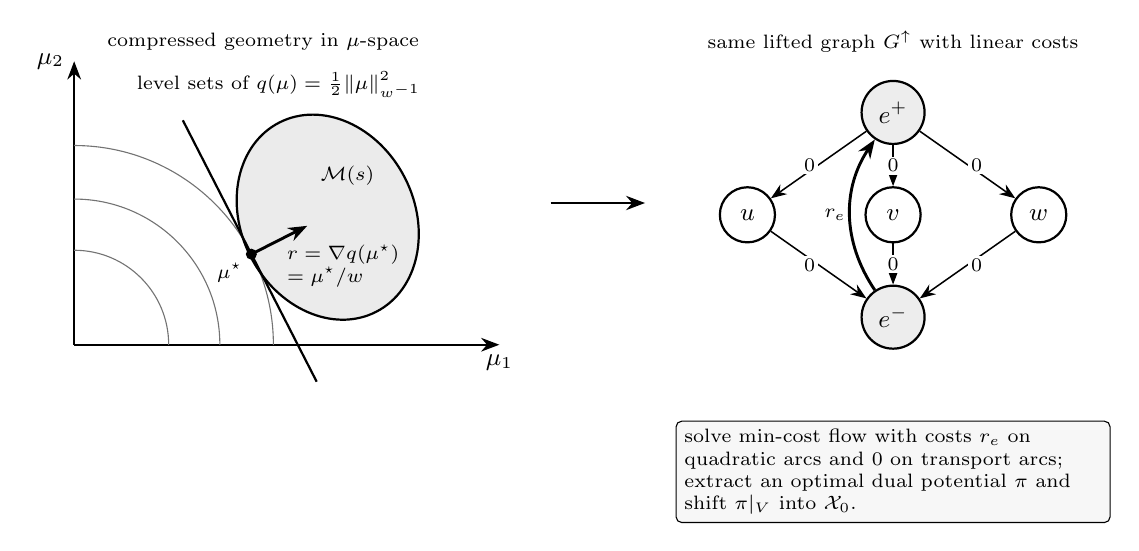
\begin{tikzpicture}[
    >=Stealth,
    x=1cm,
    y=1cm,
    every node/.style={font=\small},
    note/.style={font=\scriptsize, fill=none, inner sep=1.1pt},
    vertex/.style={circle, draw, thick, fill=white, minimum size=7mm, inner sep=0pt},
    auxnode/.style={circle, draw, thick, fill=black!7, minimum size=8mm, inner sep=0pt},
    auxarrow/.style={-{Stealth[length=2.0mm]}, line width=0.55pt},
    mainarrow/.style={-{Stealth[length=2.4mm]}, line width=1.05pt},
    costlabel/.style={font=\scriptsize, fill=white, inner sep=1pt},
    tinybox/.style={draw, rounded corners=2pt, fill=black!3, font=\scriptsize, align=left, inner sep=3pt}
  ]
  %
  \begin{scope}[shift={(0,0)}]
    \node[note] at (2.6,4.25) {compressed geometry in $\mu$-space};
    \coordinate (origin) at (0.2,0.4);
    \draw[->, thick] (origin) -- (5.6,0.4) node[below] {$\mu_1$};
    \draw[->, thick] (origin) -- (0.2,4.0) node[left] {$\mu_2$};

    \begin{scope}
      \clip (0.2,0.4) rectangle (5.6,4.0);
      \draw[thin, black!55] (origin) circle [radius=1.20];
      \draw[thin, black!55] (origin) circle [radius=1.85];
      \draw[thin, black!55] (origin) circle [radius=2.53];
    \end{scope}
    \node[note, anchor=west] at (0.95,3.70) {level sets of $q(\mu)=\tfrac12\|\mu\|_{w^{-1}}^2$};

    \coordinate (mustar) at (2.45,1.55);
    \begin{scope}[shift={(3.42,2.02)}, rotate=-62.9]
      \draw[thick, fill=black!8] (0,0) ellipse [x radius=1.35, y radius=1.10];
    \end{scope}
    \node[note] at (3.67,2.55) {$\mathcal M(s)$};

    \draw[thick] (1.58,3.25) -- (3.28,-0.07);
    \fill (mustar) circle (2pt);
    \node[note, anchor=north east] at (2.38,1.48) {$\mu^{\star}$};

    \draw[mainarrow] (mustar) -- (3.16,1.91);
    \node[note, anchor=west, align=left] at (2.86,1.4) {$r=\nabla q(\mu^{\star})$\\$=\mu^{\star}/w$};
  \end{scope}

  %
  \draw[mainarrow] (6.25,2.2) -- (7.45,2.2);

  %
  \begin{scope}[shift={(7.9,0.0)}]
    \node[note] at (2.7,4.25) {same lifted graph $G^{\uparrow}$ with linear costs};

    \node[auxnode] (ep) at (2.7,3.35) {$e^+$};
    \node[auxnode] (em) at (2.7,0.75) {$e^-$};
    \node[vertex] (a) at (0.85,2.05) {$u$};
    \node[vertex] (b) at (2.7,2.05) {$v$};
    \node[vertex] (c) at (4.55,2.05) {$w$};

    \draw[auxarrow] (ep) -- node[costlabel, left] {$0$} (a);
    \draw[auxarrow] (ep) -- node[costlabel] {$0$} (b);
    \draw[auxarrow] (ep) -- node[costlabel, right] {$0$} (c);
    \draw[auxarrow] (a) -- node[costlabel, left] {$0$} (em);
    \draw[auxarrow] (b) -- node[costlabel] {$0$} (em);
    \draw[auxarrow] (c) -- node[costlabel, right] {$0$} (em);
    \draw[mainarrow] (em) to[bend left=34] node[note, left] {$r_e$} (ep);

    \node[tinybox, below=9mm of em, text width=53mm] (potbox) {solve min-cost flow with costs $r_e$ on quadratic arcs and $0$ on transport arcs; extract an optimal dual potential $\pi$ and shift $\pi|_V$ into $\Xzero$.};
  \end{scope}
\end{tikzpicture}

\end{document}